%\chapter{models}\label{sec:models}
\section{Numerical Methods}\label{sec:models}
We made use of the public code GalIC to build the Milky Way and the
LMC initial conditions.
\subsection{Milky Way model}


In order to model the MW we use a Hernquist profile for the dark matter halo 
a exponential profile for the disk and a Hernquist profile for the bulge. For
the LMC we also use a Hernquist model. In the following subsection we explain 
in detail how the parameters of this profiles are chosen following the observational 
evidence from \verb+\citep{vandermarel14}+. 


Many groups have attempted to measure the mass of the Milky Way,
There is still no agreement. 

Therefore following \citep{Gomez15} we use three Milky Way models with
a halo, disk and bulge component. The halo masses are $M_{vir} = 1, 1.5, 
2\times 10 ^12 M\odot$, the concentration parameter are those
predicted by $\Lambda CDM$ \citep{Kyplin}. The Disk is modeled using a 
exponential disk with $R_d=3.5kpc$ and $z_0 = 0.53 kpc$ and masses
$6.5, 5.5, 5.0 \time10^{10} M_{\odot}$.
Finally the Bulge have a mass of $Mvir=1\time10^{10}M_{\odot}$ and a
scale length $r_c=0.7 kpc$, we summarize all this values in
Table\ref{tab:MWmodels}.

\begin{table}[H]{\label{tab:MW}}
\begin{center}
\begin{tabular}{c c c c c c c c c c c c}
\hline
\hline
$M_{vir} $ & $R_{vir}$ & $r_s$ & $M_{disk}$ & 10 & $M_{bulge}$ & $c_{bulge} $ & $M_{Halo}$ & $c_{halo}$ & $R_{vir, halo}$ & $M_{H,halo}$ & $r_h $ \\
\hline
100 & 261 & 26.47 & 6.5 & 3.5 & 1.0 & 0.7 & 92.5 & 9.918 &  255.82 & 135 & 53.73 \\
150 & 299 & 31.27 & 5.5 & 3.5 & 1.0 & 0.7 & 143.5 & 9.59 & 294.6 & 211  & 61.3 \\
200 & 329 & 35.15 & 5.0 & 3.5 & 1.0 & 0.7 & 194 & 9.38 & 325.8 & 289 & 69.2 \\
\hline
\end{tabular}
\caption{Summary of the Milky Way models.\lable{tab:MWmodels}}
\end{center}
\end{table}

The concentration parameter was derived using the relation from 
\verb+\citep{klypin11}+

\begin{equation}
c(M_{vir}) = 9.6(\dfrac{Mvir}{10^12 h^{-1} M\odot})^{-0.075}
\end{equation}

$c(1E12) = 9.86$, $c(1.5E12) = 9.99$, $c(2E12) = 10.12$. 

And the $R_{vir}$ is derived from:

\begin{equation}
R_{vir} = \left( \dfrac{2 G M_{vir} }{\Delta_{vir} \Omega_m H^2 } \right)^{1/3}
\end{equation}

The constants are $H = H_0 = 3.2407789E-18 h/s$ (this value of H is taken 
from GalIC) where $h=0.7$. $\Omega_m = 0.27$ and $\Delta_{vir}=360$ at $z=0$. 

\begin{figure}[H]
\centering
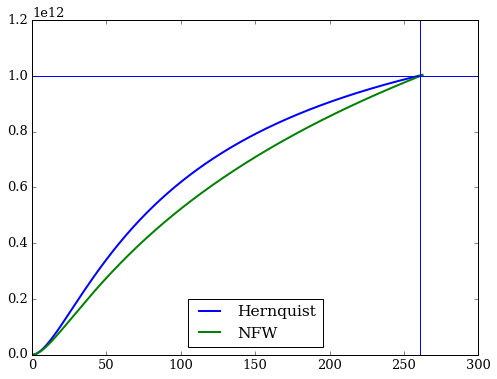
\includegraphics[scale=0.4]{MW_enclosedM.png}
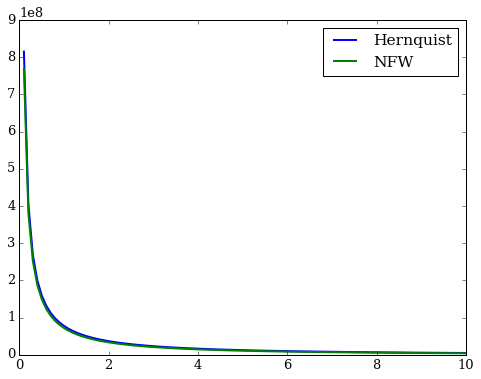
\includegraphics[scale=0.4]{MW_enclosedRho.png}
\end{figure}

The initial conditions that are the input values in the GalIC code are:

\begin{table}
\begin{tabular}{c c}
\hline
Parameter & Value \\
\hline
C & 9.91 \\
$V_vir$ & 124.76\\
\end{tabular}
\end{table}

This values comes from the code \verb+GalIC_input.py+ the code needs 
as parameter $Rvir$ and $r_s$ and it runs as follows:

\begin{verbatim}
python GalIC_input.py 9.25E11 255.8275 25.79402
\end{verbatim}

The IC corresponds to the ouput of $V_{vir}$ and $CC$, GalIC was modified 
in order to derive the Hernquist equivalence mass and the scale length for a
Hernquist profile.


\subsection{LMC models}

We model the LMC in order with the aim of reproduce the observational 
constraints in the LMC rotation curve and mass. \verb+\citep{vandermarel14}+
the rotation curve peaks at $91.7 km/s$ at $8.7 kpc$ and it remains flat 
beyond $8.7 kpc$. \verb+\citep{vandermarel14}+ also found that the enclosed
mass at $R = 8.7Kpc$ is $M(8.7) = 1.7E10$.\\

We use two different profiles a Plummer and a Hernquist to model the 
LMC. The parameters are resumed in table \ref{tab:LMC}. For these 
models the scale length is found in such a way that the enclosed 
mass  $M(9kpc) = 1.3E10$. For the Plummer model we use the value
reported by \verb+\citep{gomez15}+.



\begin{table}[H]{\label{tab:LMC}}
\begin{center}
\begin{tabular}{c c c c c c c}
\hline
\hline
$M_{LMC} (10^10M\odot)$ & 3 & 5 & 8 & 10 & 18 & 25 \\
$r_p(kpc)$ & 8 & 11 & 14 & 15 & 20 & 22.5 \\
$r_h(kpc)$ & 4.91 & 8.97 & 13.75 & 16.43 & 25.13 & 30 \\
$r_h(kpc)$ & 3.13 & 6.64 & 10.81 & 13.13 & 20.7 & 26.02 \\
\hline
\end{tabular}
\end{center}
\end{table}
%---------------------------Plummer--------------------

The enclosed mass for the Plummer profile is shown in Fig.\ref{fig:LMC_mass_p}.


\begin{figure}[H]{\label{fig:LMC_mass_p}}
\centering
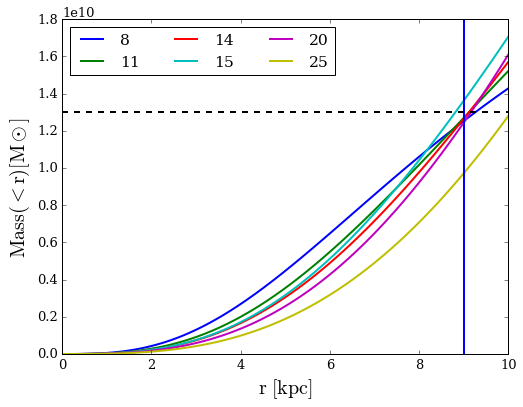
\includegraphics[scale=0.4]{LMC_mass_plummer.png}
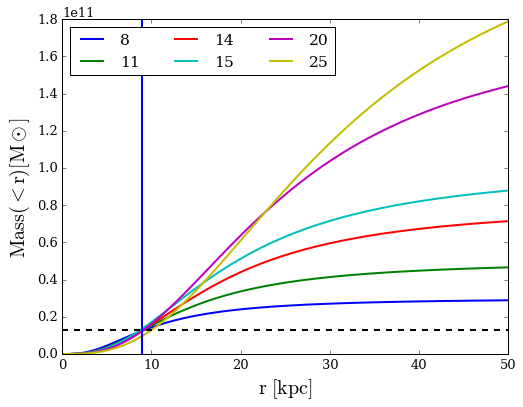
\includegraphics[scale=0.4]{LMC_mass_plummer_out.png}
\end{figure}
While the rotation curve is shown in \ref{fig:LMC_rotcurve_p}. \\
 
\begin{figure}[H]{\label{fig:LMC_rotcurve_p}}
\centering
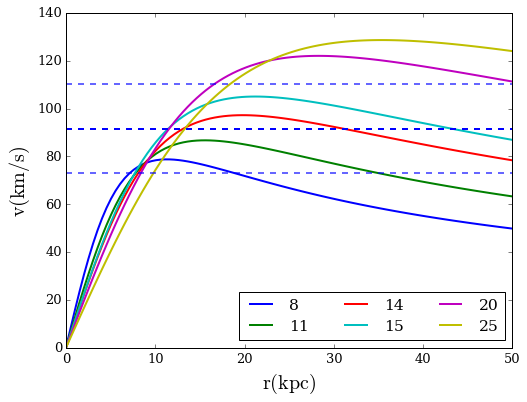
\includegraphics[scale=0.4]{LMC_rotcurve_plummer.png}
\end{figure}



%---------------------------Hernquist------------------


The enclosed mass for the Hernquist profile is shown in Fig.\ref{fig:LMC_mass}.

\begin{figure}[H]{\label{fig:LMC_mass}}
\centering
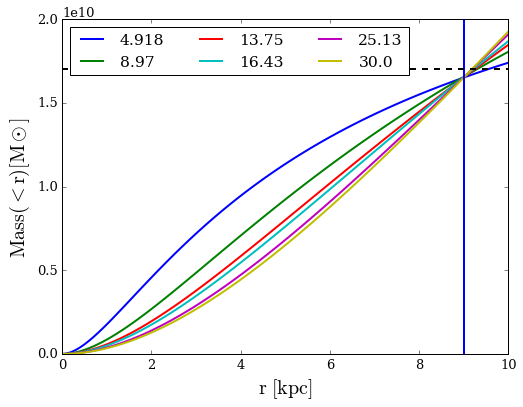
\includegraphics[scale=0.4]{LMC_mass_hernquist.png}
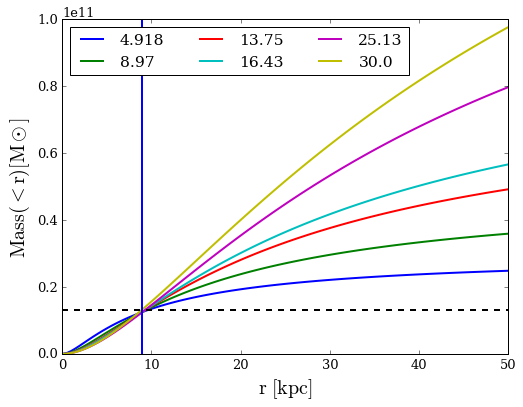
\includegraphics[scale=0.4]{LMC_mass_hernquist_out.png}
\end{figure}

While the rotation curve is shown in \ref{fig:LMC_rotcurve}.

\begin{figure}[H]{\label{fig:LMC_rotcurve}}
\centering
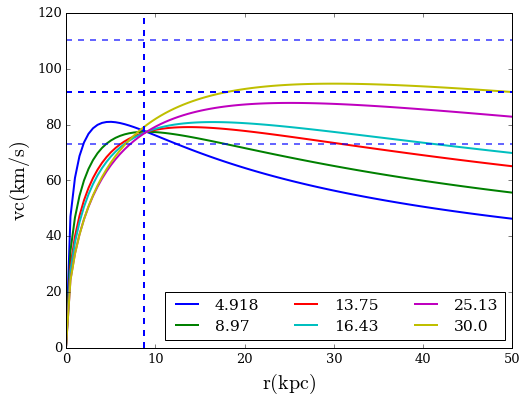
\includegraphics[scale=0.4]{LMC_rotcurve_hernquist.png}
\end{figure}


The enclosed mass for the Hernquist profile is shown in Fig.\ref{fig:LMC_mass}.

\begin{figure}[H]{\label{fig:LMC_mass}}
\centering
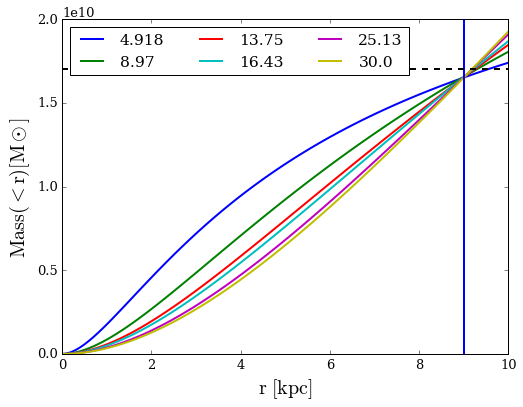
\includegraphics[scale=0.4]{LMC_mass_hernquist_2.png}
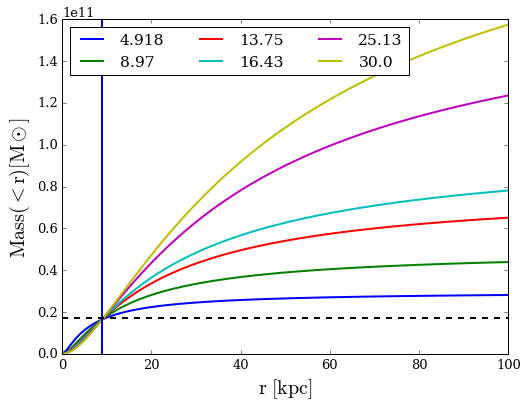
\includegraphics[scale=0.4]{LMC_mass_hernquist_out_2.png}
\end{figure}

While the rotation curve is shown in \ref{fig:LMC_rotcurve}.

\begin{figure}[H]{\label{fig:LMC_rotcurve}}
\centering
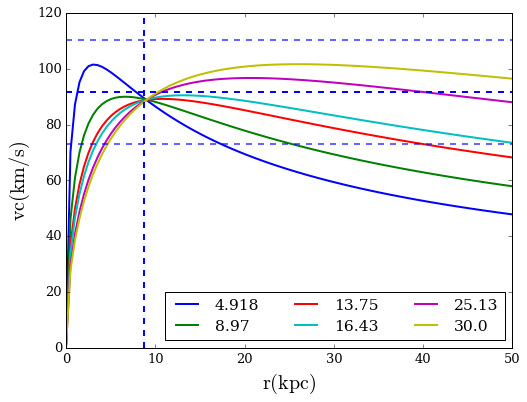
\includegraphics[scale=0.4]{LMC_rotcurve_hernquist_2.png}
\end{figure}

\subsection{GalIC modification}

In order to compute the Hernquist scale length $a$ and the Hernquist equivalent mass 
the code do the following:

\textbf{Input parameters:} CC (Halo Concentration Parameter of the NFW profile) and Vvir (Virial Velocity of the NFW halo km/s).\\
In our case this values are $M_{vir} = 1E12 M\odot$ and $CC = c_{vir} = 9.86$ \\
With these parameters we compute the \textbf{output parameters:} $M_H$ (Virial mass of the equivalent Hernquist profile) and $a$.

using:

\begin{equation}
M_{vir} = \dfrac{V_{vir}^3}{\sqrt(48.6) H G}
\end{equation}

\begin{equation}
R_{vir} = \dfrac{V_{vir}}{\sqrt(48.6)H}
\end{equation}

In the code $H = 3.2407789E-18 h / s$. \\

Which leads to $M_{vir} =  7E11 M\odot / h $ and $R_{vir} = 183.67 Kpc / h  = 262.38 kpc$ \\
 
With $R_{vir}$ and $c_{vir}$ $r_s$  could be derived: \\

\begin{equation}
r_s = \dfrac{R_{vir}} {c_{vir}} = 18.62 kpc/ h = 26.6 kpc
\end{equation} 

To get the Equivalent Hernquist mass we first we have to get the ratio $a$

\begin{equation}
a = \dfrac{r_s}{(2 f(c_{vir}))^{-1/2} - 1/c_{vir}} = 38.77 kpc/ h  = 55.38 kpc
\end{equation}

Where $f(c_{vir}) = ln(1 + c_{vir}) - c_{vir}/(1+c_{vir})$

Finally the Hernquist Mass is computed with:

\begin{equation}
M_H = \dfrac{M_{vir} (a/r_s)^2}{2f(c_{vir})} = 1.02E12 M\odot / h = 1.45E12 M\odot
\end{equation}

\subsection{Analytic:}

For the analytic we derive $M_H$ using the same procedure explained above and we get: \\

$M_H = 1.46E12 M\odot$ and  $a = 53.06 kpc$. 

Where we start from $Rvir = 261 kpc$, $r_s = 26.47$ and $M_{vir} = 1E12 M\odot$

